\documentclass[12pt]{article}

%%%%%%%%%%%%%%%%%%%%%%%%%%%%%%%%%%%%%%%%%%%%%%%%%%%%%%%%%%%%%%%%%%%%%%%%%%%%%%%%%%%%%%%%%%%%%%%%%%%%
% Math
\usepackage{fancyhdr} 
\usepackage{amsfonts}
\usepackage{amsmath}
\usepackage{amssymb}
\usepackage{amsthm}
%\usepackage{dsfont}

%%%%%%%%%%%%%%%%%%%%%%%%%%%%%%%%%%%%%%%%%%%%%%%%%%%%%%%%%%%%%%%%%%%%%%%%%%%%%%%%%%%%%%%%%%%%%%%%%%%%
% Macros
\usepackage{calc}

%%%%%%%%%%%%%%%%%%%%%%%%%%%%%%%%%%%%%%%%%%%%%%%%%%%%%%%%%%%%%%%%%%%%%%%%%%%%%%%%%%%%%%%%%%%%%%%%%%%%
% Commands and Custom Variables	
\newcommand{\problem}[1]{\hspace{-4 ex} \large \textbf{Problem #1} }
%\let\oldemptyset\emptyset
%\let\emptyset\varnothing
\newcommand{\norm}[1]{\left\lVert#1\right\rVert}
\newcommand{\sint}{\text{s}\kern-5pt\int}
\newcommand{\powerset}{\mathcal{P}}
\renewenvironment{proof}{\hspace{-4 ex} \emph{Proof}:}{\qed}
\newcommand{\solution}{\textit{Solution}:\bigbreak}
\newcommand{\RR}{\mathbb{R}}
\newcommand{\NN}{\mathbb{N}}
\newcommand{\QQ}{\mathbb{Q}}
\newcommand{\ZZ}{\mathbb{Z}}
\newcommand{\CC}{\mathbb{C}}
\newcommand{\VV}{\mathbb{V}}
\newcommand{\FF}{\mathbb{F}}
\renewcommand{\Re}{\operatorname{Re}}
\renewcommand{\Im}{\operatorname{Im}}

\newcommand{\bigO}{\mathcal{O}}

\renewcommand{\vec}[1]{\boldsymbol{\mathbf{#1}}}

\newcommand{\editnote}[1]{\textcolor{red}{\textbf{\MakeUppercase{#1}}}}


%%%%%%%%%%%%%%%%%%%%%%%%%%%%%%%%%%%%%%%%%%%%%%%%%%%%%%%%%%%%%%%%%%%%%%%%%%%%%%%%%%%%%%%%%%%%%%%%%%%%
%page
\usepackage[margin=1in]{geometry}
\usepackage{setspace}
%\doublespacing
\allowdisplaybreaks
\pagestyle{fancy}
\fancyhf{}
\rhead{Shaw \space \thepage}
\setlength\parindent{0pt}
\usepackage{color}
\usepackage{xcolor}

%%%%%%%%%%%%%%%%%%%%%%%%%%%%%%%%%%%%%%%%%%%%%%%%%%%%%%%%%%%%%%%%%%%%%%%%%%%%%%%%%%%%%%%%%%%%%%%%%%%%
%Code
\usepackage{listings}
\usepackage{courier}
\lstset{
	language=Python,
	showstringspaces=false,
	formfeed=newpage,
	tabsize=4,
	commentstyle=\itshape,
	basicstyle=\ttfamily,
}

%%%%%%%%%%%%%%%%%%%%%%%%%%%%%%%%%%%%%%%%%%%%%%%%%%%%%%%%%%%%%%%%%%%%%%%%%%%%%%%%%%%%%%%%%%%%%%%%%%%%
%Images
\usepackage{graphicx}
\graphicspath{ {images/} }
\usepackage{float}

%tikz
\usepackage[utf8]{inputenc}
%\usepackage{pgfplots}
%\usepgfplotslibrary{groupplots}

%%%%%%%%%%%%%%%%%%%%%%%%%%%%%%%%%%%%%%%%%%%%%%%%%%%%%%%%%%%%%%%%%%%%%%%%%%%%%%%%%%%%%%%%%%%%%%%%%%%%
%Hyperlinks
%\usepackage{hyperref}
%\hypersetup{
%	colorlinks=true,
%	linkcolor=blue,
%	filecolor=magenta,      
%	urlcolor=cyan,
%}

\begin{document}
	\thispagestyle{empty}
	
	\begin{flushright}
		Sage Shaw \\
		m567 - Fall 2018 \\
		\today
	\end{flushright}
	
\begin{center}{\large \textbf{Homework 4}}\end{center}
\bigbreak

%%%%%%%%%%%%%%%%%%%%%%%%%%%%%%%%%%%%%%%%%%%%%%%%%%%%%%%%%%%%%%%%%%%%%%%%%%%%%%%%%%%%%%%%%%%%%%%%%%%%
\hspace{-.5 ex}\problem{1(a)} Below is my code for solving the Poisson problem on a square domain using SOR.

\begin{lstlisting}[language=MATLAB]
function [u,x,y] = fd2poissonsor(ffun,gfun,a,b,m)
tol = 10^-8;
max_iter = 10^4;
h = (b-a)/(m+1);   % Mesh spacing
% Uniform mesh, including boundary points.
[x,y] = meshgrid(a:h:b);
idx = 2:m+1;
idy = 2:m+1;
% Compute boundary terms, south, north, east, west
ubs = feval(gfun,x(1,1:m+2),y(1,1:m+2));    % Include corners
ubn = feval(gfun,x(m+2,1:m+2),y(m+2,1:m+2));% Include corners
ube = feval(gfun,x(idy,m+2),y(idy,m+2));    % No corners
ubw = feval(gfun,x(idy,1),y(idy,1));        % No corners
% Evaluate RHS of Poisson's equation on interior points.
f = feval(ffun,x(idy,idx),y(idy,idx));
r_tol = tol * norm(f);
rhs = h^2 * f;
u = ones(m,m);
u = [ubs;[ubw,u,ube];ubn];
omega = 2/(1+sin(pi*h));
for i=1:max_iter
	for r=2:m+1
		for c=2:m+1
			u_gs = 0.25*(u(r-1,c)+u(r+1,c)+u(r,c-1)+u(r,c+1)) 
- h^2/4*f(r-1,c-1);
			u(r,c) = u(r,c) + omega*(u_gs - u(r,c));
		end
	end
	% Calculate Residual
	res = rhs + 4.* u(2:end-1, 2:end-1);
	res = res - u(1:end-2, 2:end-1);
	res = res - u(3:end, 2:end-1);
	res = res - u(2:end-1, 1:end-2);
	res = res - u(2:end-1, 3:end);
	%res = res - h^2 * f;
	if norm(res) <= r_tol
		break; 
	end
end
if i==max_iter
	warning('Max iterations reached in SOR.'); 
end
end
\end{lstlisting}
\bigbreak

This was applied to the Poisson problem given in the FD2-Poisson handout:
\begin{align*}
	\nabla^2 u(x,y) &= -5 \pi^2 \sin(\pi x)\cos(2 \pi y) \text{ for } (x,y) \in \Omega = (0,1)\times(0,1)\\
	u(x,y) &= \sin(\pi x)\cos(2 \pi y) \text{ for } (x,y) \in \partial\Omega.
\end{align*}
The resulting solution and error plot can be seen below.
\begin{figure}[H]
	\centering
	\caption{Plots of the solution and error using SOR.}
	\begin{minipage}{.5\textwidth}
		\centering
		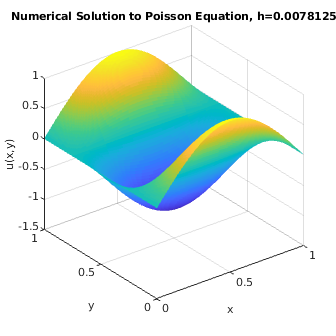
\includegraphics[width=1\linewidth]{hw4_p1_plot}
		%\captionof{figure}{A figure}
		\label{fig:test1}
	\end{minipage}%
	\begin{minipage}{.5\textwidth}
		\centering
		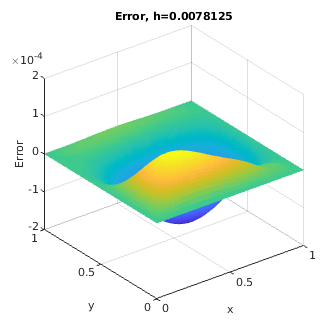
\includegraphics[width=1\linewidth]{hw4_p1_error}
		%\captionof{figure}{Another figure}
		\label{fig:test2}
	\end{minipage}
\end{figure}



\bigbreak
%%%%%%%%%%%%%%%%%%%%%%%%%%%%%%%%%%%%%%%%%%%%%%%%%%%%%%%%%%%%%%%%%%%%%%%%%%%%%%%%%%%%%%%%%%%%%%%%%%%%
\problem{2(a)} Below is my code for solving the Poisson problem on a square domain using sparse matrices.

\begin{lstlisting}[language=MATLAB]
function [u,x,y] = fd2poissonsp(ffun,gfun,a,b,m)
h = (b-a)/(m+1);   % Mesh spacing
[x,y] = meshgrid(a:h:b);   % Uniform mesh, including boundary points.
idx = 2:m+1;
idy = 2:m+1;
% Compute boundary terms, south, north, east, west
ubs = feval(gfun,x(1,1:m+2),y(1,1:m+2));     % Include corners
ubn = feval(gfun,x(m+2,1:m+2),y(m+2,1:m+2)); % Include corners
ube = feval(gfun,x(idy,m+2),y(idy,m+2));     % No corners
ubw = feval(gfun,x(idy,1),y(idy,1));         % No corners
% Evaluate the RHS of Poisson's equation at the interior points.
f = feval(ffun,x(idy,idx),y(idy,idx));
% Adjust f for boundary terms
f(:,1) = f(:,1) - ubw/h^2;             % West
f(:,m) = f(:,m) - ube/h^2;             % East
f(1,1:m) = f(1,1:m) - ubs(idx)/h^2;    % South
f(m,1:m) = f(m,1:m) - ubn(idx)/h^2;    % North
f = reshape(f,m*m,1);
% Create the D2x and D2y matrices
% Full matrix version. Can be made faster with Matlab's sparse library.
%z = [-2;1;zeros(m-2,1)];
z = ones(m,1)*[1 -2 1];
D2 = spdiags(z, [-1 0 1], m, m);
D2x = 1/h^2*kron(D2,speye(m));
D2y = 1/h^2*kron(speye(m),D2);
% Solve the system
u = (D2x + D2y)\f;
% Convert u from a column vector to a matrix to make it easier to work with
% for plotting.
u = reshape(u,m,m);
% Append on to u the boundary values from the Dirichlet condition.
u = [ubs;[ubw,u,ube];ubn];
end
\end{lstlisting}

\bigbreak
%%%%%%%%%%%%%%%%%%%%%%%%%%%%%%%%%%%%%%%%%%%%%%%%%%%%%%%%%%%%%%%%%%%%%%%%%%%%%%%%%%%%%%%%%%%%%%%%%%%%
\problem{2(b)} I have downloaded the MATLAB functions specified.

\bigbreak
%%%%%%%%%%%%%%%%%%%%%%%%%%%%%%%%%%%%%%%%%%%%%%%%%%%%%%%%%%%%%%%%%%%%%%%%%%%%%%%%%%%%%%%%%%%%%%%%%%%%
\problem{2(c)} The results of my timings are given below. These results come from running on my office computer:
\begin{table}[H]
	\caption{System Specifications}
	\begin{center}
		\begin{tabular}{|r|l|}
			\hline
			Make & Dell\\ \hline
			Processor & Intel Core i5-2400 \ \  3.10GHz x 4\\ \hline
			Memory & 7.7GiB $\approx$ 8 GB\\ \hline
			OS & Ubuntu 18.04 - Bionic Beaver\\ \hline
			Application & MATLAB - R2018a \\ \hline
		\end{tabular}
	\end{center}
\end{table}

My computer did not have enough memory to run the dense GE solver for $k=7$. Based on information from \texttt{top} - the default command line resource monitor on ubuntu (and many other systems) - it looks like my system was using around 117\% of the available memory when running this case. My system was using swap space (virtual memory) to complete the script which was dramatically increasing the runtimes. \bigbreak

The wall-clock times for GE when $k \geq 7$ are predicted times. I reasoned that GE is $\mathcal{O}(n^3)$ or in this case $\mathcal{O}((m^2)^3)$, so I did a cubic regression on $m^2$ and the wall-clock time to extrapolate. Since I needed four points for a cubic regression I also included $k=3$.

%\color{gray}
\begin{table}[H]
	\caption{Average Wall-clock time in seconds of 10 runs. {\color{gray}(predicted)}}
	\begin{center}
		\begin{tabular}{|c|c|c|c|c|c|c|}
			\hline
			$k$&$m^2$&GE&SOR&Sparse GE&DST&Multigrid\\ \hline
			3&49&0.0006967&0.0008175&0.0004143&0.0003157&0.0019262\\ \hline
			4&225&0.0037434&0.0023273&0.0007004&0.0003316&0.0030616\\ \hline
			5&961&0.018593&0.0078251&0.0015111&0.0004459&0.0052118\\ \hline
			6&3969&0.57195&0.052586&0.0056945&0.0009885&0.009997\\ \hline
			7&16129&\color{gray}41.263&0.44997&0.027005&0.0020163&0.026672\\ \hline
			8&65025&\color{gray}2808.4&4.2597&0.12434&0.0061616&0.078019\\ \hline
			9&2.6112e+05&\color{gray}1.8377e+05&38.512&0.67354&0.0324&0.41839\\ \hline
			10&1.0465e+06&\color{gray}1.1862e+07&531.5&3.0856&0.13551&2.385\\ \hline
		\end{tabular}
	\end{center}
\end{table}

\bigbreak
%%%%%%%%%%%%%%%%%%%%%%%%%%%%%%%%%%%%%%%%%%%%%%%%%%%%%%%%%%%%%%%%%%%%%%%%%%%%%%%%%%%%%%%%%%%%%%%%%%%%
\problem{2(d)} It should be noted that these predicted times for GE should be taken with a grain of salt for several reasons. Firstly, using only four points for a cubic regression and extrapolating this far outside of the range of the data is generally not going to produce meaningful results. Additionally, technical details of the hardware implementation can have great effect on the wall-clock time. In particular, solving this problem for $k=3 \implies m^2 = 49$ points probably only requires one transfer to the L1 cache. On the other hand the larger values of $k$ will require many page swaps from memory to the caches at best and in my case disk write/reads for virtual memory access. The only meaningful conclusion from these \textit{predicted} data is an example of cubic growth on $m^2$. Though the particular predicted wall-clock time for $k=10$ is not a reliable estimate, that it is roughly in the millions of seconds (weeks!) is significant. \bigbreak

Next I would like to address the seemingly poor performance of SOR. This particular implementation used MATLAB level looping to perform the updates, which is far slower than comparable operations in the libraries that MATLAB uses for vector operations and solving systems. Perhaps the rate of increase of the wall-clock times is significant, but I would not consider this an apples-to-apples comparison with the last three methods. \bigbreak

These points seem moot given the astounding speeds of the Discrete Sine Transform and Multigrid. Since the DST has order $\mathcal{O}(n\log n)) = \mathcal{O}(m^2 \log m ))$ it was expected to be among the fastest. Though Multigrid was slower it is still very impressive, particularly for an iterative method.

\bigbreak
%%%%%%%%%%%%%%%%%%%%%%%%%%%%%%%%%%%%%%%%%%%%%%%%%%%%%%%%%%%%%%%%%%%%%%%%%%%%%%%%%%%%%%%%%%%%%%%%%%%%
\problem{4(a)} Our goal is to derive the fourth-order-accurate approximation to $\Delta u = f$:
$$
\frac{1}{6h^2}\begin{bmatrix}1 & 4 & 1\\4 & -20&4\\1&4&1\end{bmatrix}u = \frac{1}{12}\begin{bmatrix} & 1 & \\1 & 8&4\\&1&\end{bmatrix}f + \mathcal{O}(h^4).
$$
To do this, we will need the following three approximations.\\
\textit{Second order approximation to $\Delta f$}:
$$
\Delta f = \frac{1}{h^2}\begin{bmatrix}&1&\\1&-4&1\\&1&\end{bmatrix}f + \mathcal{O}(h^2)
$$

\textit{Fourth order approximation to $\Delta u$}:
\begin{align}
\Delta u = \frac{1}{12h^2}\begin{bmatrix}&&-1&&\\&&16&&\\-1&16&-60&16&-1\\&&16&&\\&&-1&&\end{bmatrix}u + \mathcal{O}(h^4) \label{fourthOrder}
\end{align}

\textit{Second order approximation to $\Delta^2 u$}:
$$
\Delta^2 u = \frac{1}{h^4}\begin{bmatrix}&&1&&\\&2&-8&2&\\1&-8&20&-8&1\\&2&-8&2&\\&&1&&\end{bmatrix}u + \mathcal{O}(h^2)
$$

This last approximation can be seen by applying the Laplacian stencil recursively. That is
\begin{align*}
	\phantom{=}& \frac{1}{h^2}\left( \frac{1}{h^2}\begin{bmatrix}&&1&&\\&1&-4&1&\\&&\color{blue}1&&\\&&&&\\&&&&\end{bmatrix} +
	\frac{1}{h^2}\begin{bmatrix}&&&&\\&1&&&\\1&-4&\color{blue}1&&\\&1&&&\\&&&&\end{bmatrix} +
	\frac{1}{h^2}\begin{bmatrix}&&&&\\&&&1&\\&&\color{blue}1&-4&1\\&&&1&\\&&&&\end{bmatrix} \right.\\
	& \phantom{==}+
	\frac{1}{h^2}\begin{bmatrix}&&&&\\&&&&\\&&\color{blue}1&&\\&1&-4&1&\\&&1&&\end{bmatrix} 
	-4 \frac{1}{h^2} 
	\left. \begin{bmatrix}&&&&\\&&1&&\\&1&\color{blue}-4&1&\\&&1&&\\&&&&\end{bmatrix}
	\right)u + \mathcal{O}(h^2)= \Delta^2 u.
\end{align*}
Here the centers of the stencils have been printed in {\color{blue}blue} so that the relative position is clear. \bigbreak

We first apply the Laplacian to both sides of our PDE to obtain $\Delta^2 u = \Delta f$ and then apply our second order approximations to each side to obtain
\begin{align}
	\frac{1}{h^4}\begin{bmatrix}&&1&&\\&2&-8&2&\\1&-8&20&-8&1\\&2&-8&2&\\&&1&&\end{bmatrix}u & = 
	\frac{1}{h^2}\begin{bmatrix}&1&\\1&-4&1\\&1&\end{bmatrix}f + \mathcal{O}(h^2) \label{secondOrder}
\end{align}

Summing (\ref{fourthOrder}) + $\frac{h^2}{12}$(\ref{secondOrder}) we have
\begin{align*}
	\frac{1}{12h^2}\begin{bmatrix}2&-8&2\\-8&-40&-8\\2&-8&2\end{bmatrix}u &= 
	\frac{1}{12}\begin{bmatrix}&1&\\1&8&1\\&1&\end{bmatrix}f + \mathcal{O}(h^4)\\
	\frac{1}{6h^2}\begin{bmatrix}1 & 4 & 1\\4 & -20&4\\1&4&1\end{bmatrix}u &=
	\frac{1}{12}\begin{bmatrix} & 1 & \\1 & 8&4\\&1&\end{bmatrix}f + \mathcal{O}(h^4)
\end{align*}
as desired.

\bigbreak
%%%%%%%%%%%%%%%%%%%%%%%%%%%%%%%%%%%%%%%%%%%%%%%%%%%%%%%%%%%%%%%%%%%%%%%%%%%%%%%%%%%%%%%%%%%%%%%%%%%%
\problem{4(b)}

\bigbreak
%%%%%%%%%%%%%%%%%%%%%%%%%%%%%%%%%%%%%%%%%%%%%%%%%%%%%%%%%%%%%%%%%%%%%%%%%%%%%%%%%%%%%%%%%%%%%%%%%%%%
\problem{4(c)}

\bigbreak
%%%%%%%%%%%%%%%%%%%%%%%%%%%%%%%%%%%%%%%%%%%%%%%%%%%%%%%%%%%%%%%%%%%%%%%%%%%%%%%%%%%%%%%%%%%%%%%%%%%%
\problem{5(a)} Consider the function $f(u,t) = |u|$ on $\mathcal{D}=[-1,1] \times (-\infty, \infty)$. Is $f$ continuous with respect to $u$ on $\mathcal{D}$? \bigbreak

\textit{Claim:} Yes, it is in fact uniformly continuous with respect to $u$. \bigbreak

\begin{proof}
	Let $t \in (-\infty, \infty)$. Let $\delta >0$. Choose $\varepsilon = \delta$. Let $u, u^* \in [-1, 1]$ such that $\vert u - u^* \vert < \delta$. Then 
	\begin{align*}
		\vert f(u, t) - f(u^*,t) \vert &= \big \vert \vert u \vert - \vert u^* \vert \big \vert  \\
		& \leq \vert u - u^* \vert \tag{reverse triangle inequality} \\
		& \leq \delta = \varepsilon.
	\end{align*}
\end{proof}

\bigbreak
%%%%%%%%%%%%%%%%%%%%%%%%%%%%%%%%%%%%%%%%%%%%%%%%%%%%%%%%%%%%%%%%%%%%%%%%%%%%%%%%%%%%%%%%%%%%%%%%%%%%
\problem{5(b)} Is $f$ Lipschitz continuous with respect to $u$ on $\mathcal{D}$? \bigbreak

\textit{Claim:} Yes, it is Lipschitz with constant $L = 1$. \bigbreak

\begin{proof}
	Let $t \in (-\infty, \infty)$. Let $\delta >0$. Choose $\varepsilon = \delta$. Let $u, u^* \in [-1, 1]$ such that $\vert u - u^* \vert < \delta$. Then 
	\begin{align*}
		\vert f(u, t) - f(u^*,t) \vert &= \big \vert \vert u \vert - \vert u^* \vert \big \vert  \\
		& \leq \vert u - u^* \vert. \tag{reverse triangle inequality}
	\end{align*}
\end{proof}

\bigbreak
%%%%%%%%%%%%%%%%%%%%%%%%%%%%%%%%%%%%%%%%%%%%%%%%%%%%%%%%%%%%%%%%%%%%%%%%%%%%%%%%%%%%%%%%%%%%%%%%%%%%
\problem{5(c)} Is the initial value problem 
$$
u'(t) = \vert u \vert, \phantom{=} -1 \leq t \leq 1, \phantom{=}u(-1)=-1
$$
well-posed? \bigbreak

\textit{Claim:} Yes, it is well posed. \bigbreak

\begin{proof}
	The function $f(u,t) = \vert u \vert$ is obviously continuous in $t$. \bigbreak
	
	As stated in part (b), $f(u,t) = \vert u \vert$ is Lipschitz on the domain $\mathcal{D}=[-1,1] \times (-\infty, \infty)$. The same proof can be used to show that it is Lipschitz on $\mathcal{D}=[a,b] \times [-1,1]$ for any closed interval $[a,b]$. \bigbreak
	
	By our Existence and Uniqueness Theorem we have that the IVP has a unique solution for $t \in [-1, 1]$.
\end{proof}

\end{document}
